%particles
\newcommand{\jpsi}{\rm J/$\psi$}
\newcommand{\psip}{$\psi^\prime$}
\newcommand{\jpsiDY}{\rm J/$\psi$\,/\,DY}
\newcommand{\chic}{$\chi_{\rm c}$}
\newcommand{\pip}{$\pi^{+}$}
\newcommand{\pim}{$\pi^{-}$}
\newcommand{\pizero}{$\pi^{0}$}
\newcommand{\kap}{K$^{+}$}
\newcommand{\kam}{K$^{-}$}
\newcommand{\pbar}{$\rm\overline{p}$}
\newcommand{\ccbar}{\ensuremath{\mathrm{c\overline{c}}}}
\newcommand{\bbbar}{\ensuremath{\mathrm{b\overline{b}}}}
\newcommand{\Dzero}{\ensuremath{\mathrm{D^{0}}}}
\newcommand{\Dzerobar}{\ensuremath{\mathrm{\overline{D}^{0}}}}
\newcommand{\Dpm}{\ensuremath{\mathrm{D^{\pm}}}}
\newcommand{\Ds}{\ensuremath{\mathrm{D_{s}^{\pm}}}}
\newcommand{\Dstar}{\ensuremath{\mathrm{D^{*\pm}}}}

%collision systems
\newcommand{\pp}{pp}
\newcommand{\pPb}{p--Pb}
\newcommand{\PbPb}{Pb--Pb}

%detectors
\newcommand{\ezdc}{$E_{\rm ZDC}$}

%units
\newcommand{\GeVc}{GeV/$c$}
\newcommand{\GeVcsq}{GeV/$c^2$}

%others
\newcommand{\degree}{$^{\rm o}$}
\newcommand{\s}{\ensuremath{\sqrt{s}}}
\newcommand{\snn}{\ensuremath{\sqrt{s_{\rm NN}}}}
\newcommand{\y}{\ensuremath{y}}
\newcommand{\pt}{\ensuremath{p_{\rm T}}}
\newcommand{\dedx}{d$E$/d$x$}
\newcommand{\dndy}{d$N$/d$y$}
\newcommand{\dndydpt}{${\rm d}^2N/({\rm d}y {\rm d}p_{\rm t})$}
\newcommand{\zpar}{\ensuremath{z_{||}}}
\newcommand{\zpargen}{\ensuremath{z_{||}^{\mathrm{part}}}}
\newcommand{\zpardet}{\ensuremath{z_{||}^{\mathrm{det}}}}
\newcommand{\ptchjet}{\ensuremath{p_{\mathrm{T,ch\, jet}}}}
\newcommand{\ptjet}{\ensuremath{p_{\mathrm{T,jet}}}}
\newcommand{\ptchjetgen}{\ensuremath{p_{\mathrm{T,ch\,jet}}^{\mathrm{part}}}}
\newcommand{\ptchjetdet}{\ensuremath{p_{\mathrm{T,ch\,jet}}^{\mathrm{det}}}}
\newcommand{\ptd}{\ensuremath{p_{\mathrm{T,D}}}}
\newcommand{\ptdgen}{\ensuremath{p_{\mathrm{T,D}}^{\mathrm{part}}}}
\newcommand{\ptddet}{\ensuremath{p_{\mathrm{T,D}}^{\mathrm{det}}}}
\newcommand{\antikt}{anti-\ensuremath{k_{\mathrm{T}}}}
\newcommand{\Antikt}{Anti-\ensuremath{k_{\mathrm{T}}}}
\newcommand{\kt}{\ensuremath{k_{\mathrm{T}}}}
\newcommand{\pthard}{\ensuremath{p_{\mathrm{T,hard}}}}
\documentclass[12pt, a4paper, twoside, titlepage]{article}
% font size could be 10pt (default), 11pt or 12 pt
% paper size coulde be letterpaper (default), legalpaper, executivepaper,
% a4paper, a5paper or b5paper
% side coulde be oneside (default) or twoside 
% columns coulde be onecolumn (default) or twocolumn
% graphics coulde be final (default) or draft 
%
% titlepage coulde be notitlepage (default) or titlepage which 
% makes an extra page for title 
% 
% paper alignment coulde be portrait (default) or landscape 
%
% equations coulde be 
%   default number of the equation on the rigth and equation centered 
%   leqno number on the left and equation centered 
%   fleqn number on the rigth and  equation on the left side
%
\usepackage{hyperref}
\usepackage{graphicx}  % needed for figures
\usepackage{dcolumn}   % needed for some tables
\usepackage{bm}        % for math
\usepackage{amssymb}   % for math
\usepackage{amsfonts}
\usepackage{graphics}
\usepackage{grffile}   % to handle dots in graphics file names
\usepackage{epsfig}
\usepackage{units}
\usepackage{comment}
\usepackage[usenames]{color}
\usepackage[normalem]{ulem} % for strikethroughs (\sout{})
\usepackage{color}
\usepackage[utf8]{inputenc}
\usepackage[T1]{fontenc}
\usepackage{subfigure}
\usepackage{multirow}
\usepackage{tablefootnote}
\title{Measurement of charm jet cross-section and fragmentation function
with the ALICE detector at the LHC}
\author{Salvatore Aiola  \\
	Advisers: John Harris, Helen Caines \\
	Yale University Physics Department
	}

\date{\today} 
% \date{\today} date coulde be today 
% \date{25.12.00} or be a certain date
% \date{ } or there is no date 
\begin{document}
% Hint: \title{what ever}, \author{who care} and \date{when ever} could stand 
% before or after the \begin{document} command 
% BUT the \maketitle command MUST come AFTER the \begin{document} command! 
\maketitle

\begin{abstract}
Jets are a fundamental feature of high-energy particle interactions. 
They result from the fragmentation of hard-scattered partons, 
a key process of Quantum Chromodynamics (QCD). 
In particular, the production and the internal properties of heavy-flavor jets 
in pp collisions are not yet satisfactorily described by neither analytical nor 
phenomenological approaches to QCD. Measurements are needed
in order to provide important constraints to models inspired by perturbative QCD 
and Monte-Carlo generators, such as PYTHIA and POWHEG, widely used in high-energy particle physics.

Heavy-flavor jets can also provide important insights into the Quark-Gluon Plasma (QGP)
produced in ultra-relativistic heavy-ion collisions, as heavy quarks are predicted
to interact with the QGP differently compared to light quarks and gluons. 
However, their production mechanisms must first be studied in the vacuum, 
in order to provide a baseline for the observation of possible modifications induced by the presence of the QGP. 

We present the current status of the measurement of jets that contain a D meson (D-tagged jet) with \mbox{ALICE}.
The aim of the analysis is to extract both the $p_{\rm T}$ spectrum of the D-tagged jets and the jet-momentum fraction of the D mesons. 
We identify D-meson candidates via their hadronic decay channels using topological selections and particle identification.
These D-meson candidates are combined with the other charged tracks reconstructed by the central tracking system, 
using the anti-$k_{\rm T}$ jet-finding algorithm.
We extract the yield of D-tagged jets through an invariant mass analysis of the D-meson candidates associated with each jet, 
in bins of jet $p_{\rm T}$ and momentum fraction carried by the D meson. Finally we use a standard unfolding procedure 
to correct the jet $p_{\rm T}$ spectrum for detector inefficiencies and momentum resolution. For this analysis we use data collected
by ALICE with minimum bias triggers in pp collisions at 7 TeV. We will discuss also
the perspectives for the same measurement in Pb--Pb and p--Pb collisions.
\end{abstract}

%\tableofcontents % create a table of contents 

\section{Introduction}
The \emph{charm} quark was discovered in 1974 almost simultaneously by two groups, working at SLAC~\cite{Richter:1974} and at BNL~\cite{Ting:1974}.
The two groups observed a new resonance with a mass of about 3.1 \GeVcsq\ decaying into a pair of leptons.
The decay width was measured as being smaller than experimental precision; this feature
was in itself a strong indication of the existence of a new quantum number, conserved by strong nuclear interactions 
but violated in electro-weak processes.
The resonance later became known with the double name \jpsi\ and was identified as one of the possible bound states
of a new heavier quark, \emph{charm}, and of its corresponding anti-particle. 
\begin{comment}
A few years later (1977) an even heavier quark, the \emph{bottom} quark,
was discovered~\cite{Lederman:1977}; the sixth and last known quark, \emph{top}, took a bit longer (1995), due to its comparatively huge mass of about 173 \GeVcsq~\cite{CDF:1995,D0:1995}.
\end{comment}

\begin{figure}[tbh]
\begin{center}
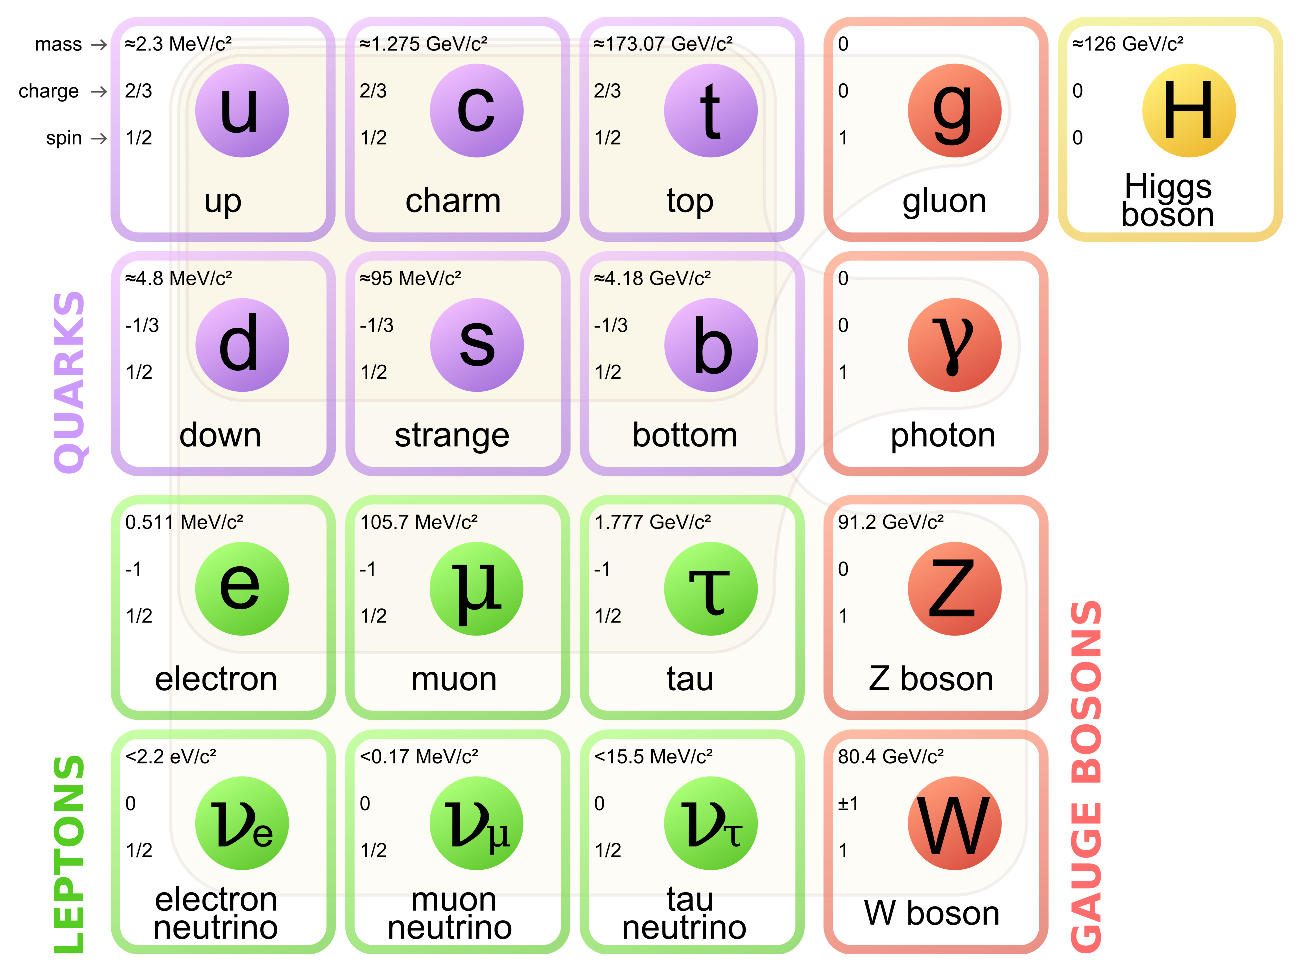
\includegraphics[width=0.8\textwidth]{img/standard_model}
 \caption{Standard Model of Particle Physics~\cite{Wikipedia:StandardModel}.} 
 \label{fig:standard_model}
\end{center}
\end{figure}

Figure~\ref{fig:standard_model} shows an illustration of the Standard Model, which includes
3 generations of leptons (electron, muon, tau), 3 generations of quarks, 4 interaction bosons, ($\gamma$, Z, $\mathrm{W}^{\pm}$, g) and the Higgs boson
recently observed by the ATLAS and CMS Collaborations \cite{ATLAS:2012b,CMS:2012d}.
Each generation of particles (either quarks or leptons) differs from the others for the strength of its coupling to the Higgs boson,
which result in a different observed mass.

At hadron colliders charm quarks are produced as a result of a parton hard scattering. Likewise lighter quarks or gluons, charm quarks
fragment into collimated sprays of hadrons called jets. The charm content of the jet is conserved throughout the fragmentation process,
which is dominated by Quantum Chromo-Dynamics, the theory of strong nuclear interactions.
The charm content of a jet can be identified looking for the presence of charmed hadrons, i.e. hadrons that have
a charm quark among their valence quarks. Since all charmed hadrons have short lifetimes ($\tau \lesssim 10^{-12}$~s) their presence is inferred
using a combination of Particle Identification (PID) techniques and topological and kinematical pattern selections on their decay products.

Charm jets have peculiar properties that result form the heavier mass of the originating parton (a charm quark).
Their production cross-section is significantly smaller than lighter quarks or gluons. The internal
properties of the jets are also affected, in particular the fragmentation is expected to be harder for charm jets compared to inclusive jets.

An observable of interest is the relative fraction of charm jets with respect to all jets. Another important observable is the fraction of the jet momentum carried by
the charmed hadron(s). Few measurements have been performed, 
with large uncertainties and/or limited kinematical reach~\cite{}. Theoretical descriptions are lacking~\cite{}, whereas commonly used Monte Carlo particle
generators, such as PYTHIA~\cite{Sjostrand:2006} or POWHEG~\cite{}, fail to reproduce the measurements~\cite{}. 
This poses problems for the High Energy Physics community since these Monte Carlo generators are widely employed as input for detector response simulations.

Heavy quarks are also an ideal probe~\cite{} of the hot and dense matter, known as Quark-Gluon Plasma (QGP)~\cite{}, that is created in ultra-relativistic heavy-ion collisions. 
Hard scattered partons, including heavy quarks, are produced early in the collision. They interact with the QGP, which increases their virtuality and interferes with the
parton fragmentation process. This effect, known as \emph{jet quenching}, leads to a broadening and softening of the jet fragmentation~\cite{}. A number of
experimental evidences of jet quenching have been produced in last decade~\cite{}.
High-energy charm jets behave very much like jets originated by light quarks~\cite{}; however at lower energies, comparable to the charm quark mass, the charm quark is expected
to interact less strongly with the QGP, a phenomenon known as dead-cone effect~\cite{}. The difference between the interaction of a light quark with the QGP and that of
a charm quark is driven by its mass, and is similar to the difference observed in Quantum Electro-Dynamics between muons and electrons interacting with regular matter.

Charm quarks are produced abundantly at the \emph{Large Hadron Collider}, which provides \pp, \pPb\ and \PbPb\ collisions at unprecedented high collision energies and luminosities.
At the LHC, the PID and low-momentum tracking capabilities are among the strongest points of ALICE~\cite{} compared to the other LHC experiments; 
this advantage is counterbalanced by an overall slower detector which does not allow to probe the full luminosity delivered by the LHC. 
Especially vertexing, tracking and PID are crucial to efficiently identify the decay products of charmed hadrons; tracking and calorimetry are used together to reconstructed the energy flow from which jets can be identified.
ALICE is very well endowed to perform a precise measurement of charm jets in a (mostly) unexplored kinematical region. Furthermore ALICE performances
are optimized for heavy-ion collisions, where charm jet measurements can provide important insights about the QGP.

\section{The Large Hadron Collider}
The \emph{Large Hadron Collider} (LHC) at CERN is the world's largest particle collider ever built.
It is housed in a tunnel with a circumference of 27 km, between 50 and 175 m beneath
the France-Switzerland border near the city of Geneva. The tunnel was built in the 1980s and was used until 
the late 1990s to house the Large Electron-Positron Collider (LEP). The construction of the LHC took about 10 years and started
during the decommissioning phase of LEP. 

Two parallel beam pipes run through the tunnel,
where particles are allowed to travel in opposite directions, intersecting at four points where four different experiments
can detect and measure the collisions (\mbox{ATLAS}, \mbox{ALICE}, \mbox{CMS}, \mbox{LHCb}). More than 1,000 superconducting dipole magnets
are used to keep the particles in their circular trajectories, plus about other 400 superconducting quadrupole and higher multipole
magnets, which are needed to keep the beams focused and provide other optical corrections.

Protons and lead ions undergo several pre-acceleration steps before being injected into the LHC at the energy of 900 GeV.
They are injected in bunches, spaced by 25 ns (or multiple of it) for a maximum of 2,808 bunches when operating at full luminosity in \pp\ collision mode.
Acceleration is provided through radio frequency cavities. At it highest energy (currently 6.5 TeV) the dipole magnets need to generate
a magnetic field of 7.7 T.

At time of writing (July 2016) the LHC is in its Run-2 phase. The first operational phase of the LHC (Run-1) started in November 2009 and was 
concluded in February 2013. In this first phase the LHC successfully provided \pp, \pPb\ and \PbPb\ collisions.
Between 2013 and 2015 the LHC operations were stopped to allow for upgrades to the machine and to the four experiments (Long Shutdown 1, or LS1).
Run-2 started in April 2015 and is scheduled to extend till the end of 2018. Table~\ref{tab:LHCop} shows details of the LHC operations in Run-1 and Run-2.
After Run-2 another 2-year stop is foreseen (LS2) to allow for more upgrades, before the third operational phase (scheduled to start in 2021).

\begin{table}
\centering
\begin{tabular}[tbh]{lrr}
Collision system	&	Years		&	\s\ (TeV)	\\
\hline
\hline
\\
\multicolumn{3}{l}{Run-1} \\
\hline
\multirow{4}{*}{\pp}	&	2009			&	0.9		\\
				&	2010, 2011	&	7		\\
				&	2011			&	2.76		\\
				&	2012			&	8		\\
\hline
\PbPb			&	2010, 2011	&	2.76 		\\
\hline
\pPb				&	2012\tablefootnote{Pilot run}, 2013	&	5.02	\\
\hline
\\
\multicolumn{3}{l}{Run-2} \\
\hline
\multirow{2}{*}{\pp}	&	2015, 2016				&	13	\\
				&	2015						&	5.02	\\
\hline
\PbPb			&	2015						&	5.02	\\
\hline
\pPb				&	2016\tablefootnote{Planned}		&	5.02	\\
\hline
\end{tabular}
\caption{LHC Run-1 and Run-2 operations.
\label{tab:LHCop}}
\end{table}

\section{The ALICE Experiment}
ALICE (\emph{A Large Ion Collider Experiment}) is the experiment dedicated to heavy-ion collisions at the LHC.


\section{D-tagged jets with ALICE}
\subsection{Physics goals}
\subsection{Analysis technique}
\subsection{Preliminary results}
\subsection{Timeline}
\bibliography{biblio}{}
\bibliographystyle{utphys}

\end{document}
